\chapter{Pupil Detection}
\label{chap:pupildetection}
It would be very difficult to improve an algorithm, if there were no test data available. The generated pictures of the last chapter lay the foundation to improve the algorithm to detect the pupil digitally.

This chapter shows how the current algorithm tries to detect a pupil. Improvements are presented that achieve a better result.
\section{Overview of Existing Algorithm}
The general sequence of the algorithm can be described as follows:
\begin{enumerate}
	\item Find the darkest spot
	\item Extract rays starting from the darkest spot from the image
	\item Transit the rays with a filter of certain length to detect edges
	\item Fit an ellipse on the detected edges with the least square method
\end{enumerate}
The darkest spot is determined by a raster with a fixed distance between points. For each point the average with the surrounding eights point is calculated. The point with the darkest average is the start point for the rest of the algorithm.

Outgoing from the start point, rays are stamped out by the sturstarburst \gls{IP}. For more information about the starburst \gls{IP}, visit "Eye Tracking For Sports, Chapter 18.5"\cite{retoDamian}.

The difference to the next pixel is calculated for each ray that is stamped out by the starburst \gls{IP}. A filter is applied that adds multiple neighbouring differences together to build a score for each pixel. The pixel with the highest score is a detected edge.

Every edge point is handed over to a weighted least square method to find an ellipse that fits the points well. The residuals of the lest square fitting are used to calculate how well the ellipse fits on the points. \cite{retoDamian}

\subsubsection{Testing}
The algorithm was tested with pictures that were inserted at compile time. The output of the algorithm was then compared with the input picture. This is not efficient and is addressed in the next section.
\section{Improve Testing}
\label{sec:improveTesting}
It is very time consuming to generate picture data that can be compiled. After that the output of the program still needs to be compared with the input picture. A simpler way would ba a tool that can read a video file and display the result of the algorithm on each picture.

The program "Gazelle View" that was developed during the project study can already open and play video files. Because of the modular design of Gazelle View it is simple to insert the algorithm during the decode phase and paint the rays, the detected edges and the fitted ellipse on the image.

All data that was produced by the algorithm may also hold information about bugs. Such data also helps by analysing problems with the algorithm.
So every information that the algorithm generates is displayed beside each frame.

The next step to improve testing would be to automate it and condense the performance of the algorithm to parameters such as the mean and standard deviation of the accuracy.

This should be done on a wide variety of test data. Ideally, with high frame rate pictures that were captured with the eye-tracking system. For each of those pictures, an ellipse has to be fitted manually and stored as a reference. Because this needs to be done for a lot of pictures, the process of generating the reference should to be simplified.

\section{Outliers}
The supplied algorithm does not differentiate between edges that are from the pupil, hair or the eyelid. The algorithm works fine when every edge is a correct one as seen in figure \ref{fig:oldGood}. But as a consequence to the least square method, a single false detection severely alters the fitted ellipse. Such a case can be observed in figure \ref{fig:oldOutlier}. 
\begin{figure}
	\begin{subfigure}{.5\textwidth}
		\centering
		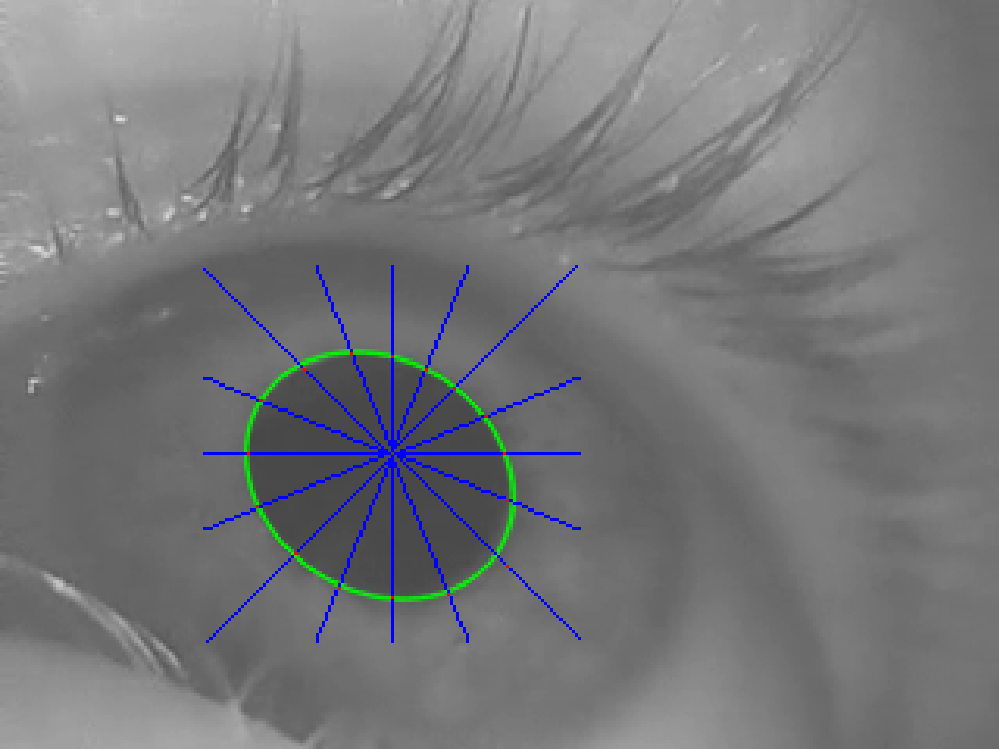
\includegraphics[width=\linewidth]{images/good_fit_old.png}
		\caption{Fitting of Ellipse without outliers}
		\label{fig:oldGood}
	\end{subfigure}%
	\begin{subfigure}{.5\textwidth}
		\centering
		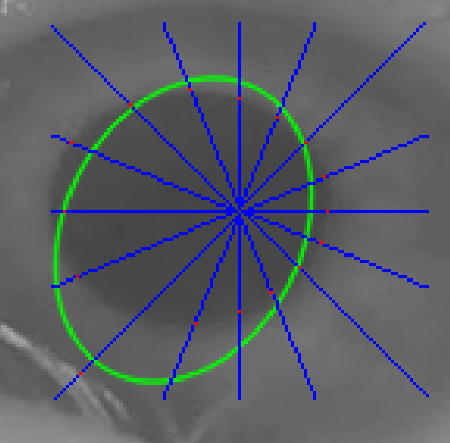
\includegraphics[width=.8\linewidth]{images/outlier_problem.png}
		\caption{Fitting of Ellipse with one outlier}
		\label{fig:oldOutlier}
	\end{subfigure}
\caption{Comparison between results with and without an outlier. It shows the big impact of an outlier on the least square fitting.}

\end{figure}

To minimize the influence of outliers there occurrence needs to be reduced. Additionally, outliers should be detected so they can be ignored.

\section{Angle-Validation}
\label{sec:angleValidation}
To detect outliers it is necessary to find properties that differ strongly from the other edges. One of those properties gets visible when the angle for each edges gets calculated with the neighbouring edges.

In figure \ref{fig:outlierOutside} an outlier is in the bottom left corner, outside of the pupil. The angle of the outlier is very small compared to the angle of neighbouring edges. Those on the other hand have a larger angle than the other edge points.

When an outlier is inside the pupil then the situation is reversed as visible in figure \ref{fig:outlierInside} where the outlier has a large angle and the adjacent edges very small angles.

\begin{figure}[H]
\begin{subfigure}{.33\textwidth}
	\centering
	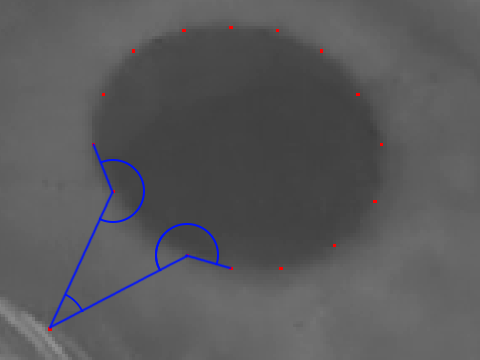
\includegraphics[width=.8\linewidth]{images/angle.png}
	\caption{Outlier outside Pupil}
	\label{fig:outlierOutside}
\end{subfigure}%
\begin{subfigure}{.33\textwidth}
	\centering
	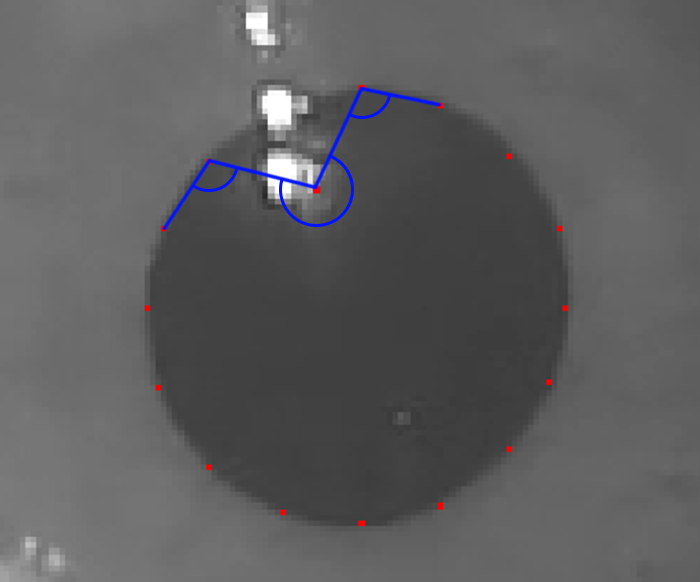
\includegraphics[width=.8\linewidth]{images/outlier_inner.png}
	\caption{Outlier inside Pupil}
	\label{fig:outlierInside}
\end{subfigure}
\begin{subfigure}{.33\textwidth}
	\centering
	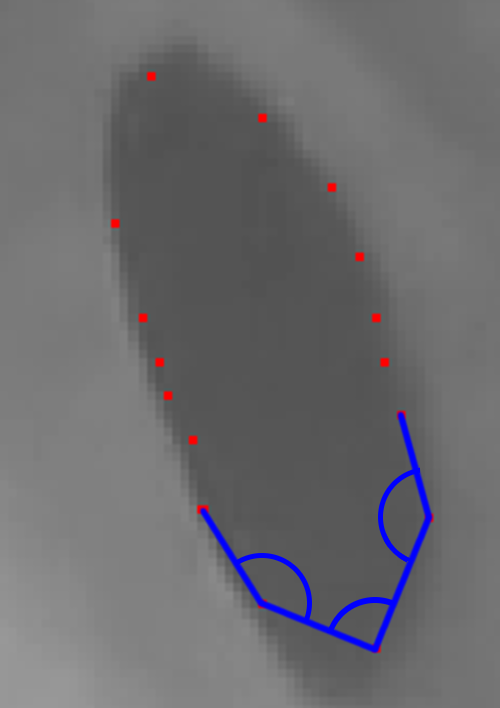
\includegraphics[width=.6\linewidth]{images/non_outlier.png}
	\caption{Accurate Transitions  with small Angles}
	\label{fig:nonOutlier}
\end{subfigure}
\caption{Angles between edges around possible outliers}
\end{figure}

Multiple adjacent outliers differ in that it is not possible to make a clear statement what the angle will be. But the neighbours to outliers still have the same properties as described in the last paragraphs. For that reason an algorithm that wants to detect outliers should focus on detecting the neighbours of outliers.

In figure \ref{fig:nonOutlier} three adjacent edges have angles that appear too small compared to its neighbours. None of them are outliers.

\subsubsection{Overview of Algorithm}
\label{sec:descriptionOfAngleValidation}

The algorithm to detect outliers based on the angles between edges involves four steps:

\begin{enumerate}
	\item Calculate angles
	\item Find 3 adjacent angles with small differences
	\item Categorize angles
	\begin{itemize}
		\item To big
		\item To small
		\item As expected 
	\end{itemize}
	\item Determine outliers
\end{enumerate}
\subsubsection{Calculate Angles}
\label{sec:calculateAngles}
The angle between the points is calculated with the vectors that stretch from the center point to the other points. For each vector the angle between the x axis and the vector is calculated with the \gls{atan2} function. The difference between the resulting two angles is the searched angle.

When the detected edges are close to each other, measurement uncertainty can greatly affect the angles at such points. To mitigate that effect the angle for a point is only calculated with transitions that are distant enough.
\subsubsection{Find Adjacent Angles With Small Differences}
Context is important to categorize an angle. Only angles that are as expected do not always require context. This is the case when there are three adjacent angles that fall within a narrow range of each other and create context for the neighbouring angles.

\subsubsection{Categorize Angles}
The found context leads the way to iterate over every edge and categorize the angle within the context. This is done as described in the decision making diagram in \ref{fig:decisionMaking}. Angles are classified into three groups. Angles that are as expected, too big or too small. 

\begin{figure}[H]
	\centering
	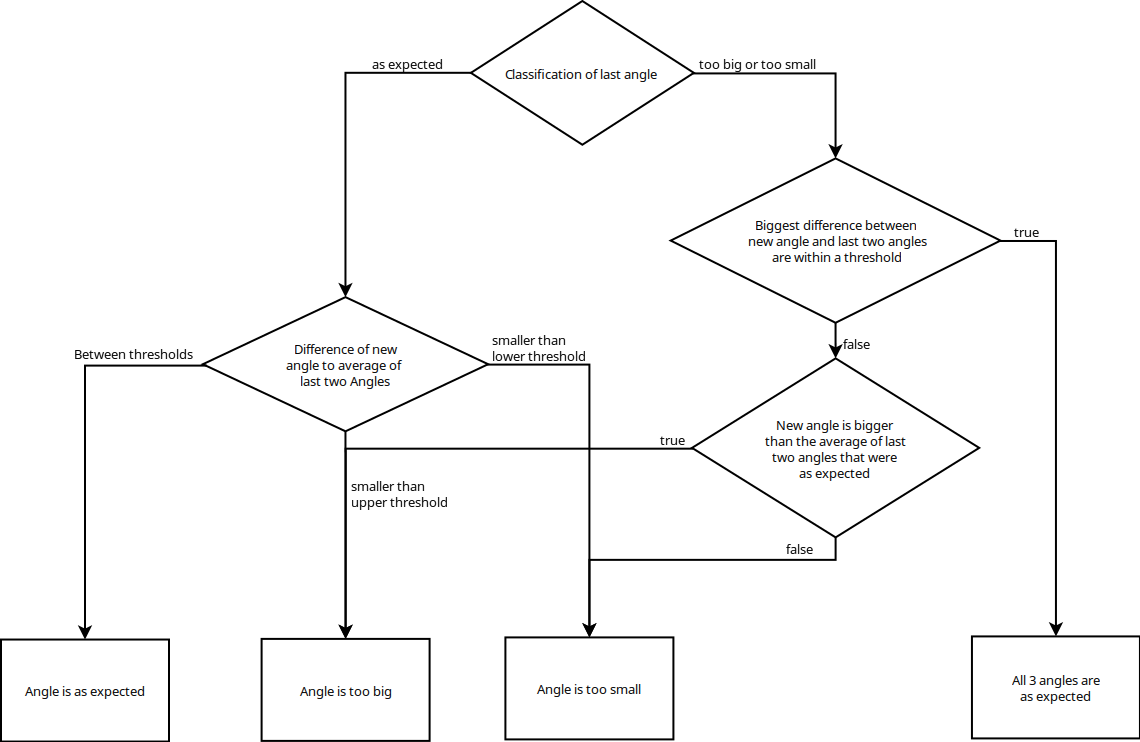
\includegraphics[width=.9\linewidth]{images/angleclassification.png}
	\caption{Decision making diagram for categorizing angles. Note that previous categorization might be overwritten by a later decision}
	\label{fig:decisionMaking}
\end{figure}
\subsubsection{Determine Outliers}
As described in section \ref{sec:angleValidation} outliers are surrounded by angles that are not as expected. The categorized angles make that determination straight forward. An outlier is an edge where neither the angle before or after is categorized as expected. 
The situation shown in figure \ref{fig:nonOutlier} constitutes an exception to this rule. This exception only occurs with adjacent small angles with neighbours that are as expected. 
\section{Colour of the Startpoint}
\label{sec:colorStartpoint}
The pupil has an uniform colour. So edges that transit from the pupil to the iris start with a colour close to the colour of the start point. Edges between the iris and the eyelid start with a colour that is brighter. This correlation can be exploited to improve the number of correctly detected transitions. By dividing the score during the filter with the difference between the colour of the beginning of the edge and the start point. To avoid a division with zero the absolute difference with an offset is used. The offset can also be used to control the influence of this part of the algorithm. 
\section{Border Detection}
\label{sec:randdetektion}
The colours of the starburst are represented by the values between one and 255. When a point of the starburst is outside the image, then it is set to zero. With that it is simple to detect the border. The behaviour in this case is different depending if there was already an edge or not. If there was already an edge we would like to keep that edge otherwise the result of this ray should be discarded.

To decide if an edge has already occurred a similar method as in section \ref{sec:colorStartpoint} is used. But a hard threshold is applied isntead of adjusting the score.
\section{Exploit good Results}
\label{sec:goodResults}

The high frame rate of the eye-capturing cameras results in small differences of the pupil position between frames. This can be used to improve the result because we already have an idea what the ellipse will look like. The start point can be adjusted to be the center of the old ellipse so the detected edges will be more equally distributed.

With the old ellipse it is also possible to calculate where a ray would transit this ellipse. This information is used to weight the score of a transition similar as the colour of the start point in section \ref{sec:colorStartpoint} was handled. The score is divided by the absolute distance in pixel to the old ellipse on the ray with a small offset.

\section{Fixed Threshold}
\label{sec:fixedThreshold}
This section is about a method that replaces the ray transition that uses a filter with a threshold.

An edge is detected when the difference to the colour of the start point is greater than a certain threshold.

As shown in chapter \ref{chap:results} this produces better result than the filter. But it is possible that the fixed threshold causes problems under certain light conditions. Further analysis is needed to evaluate that risk. But even if it turns out to be a problem, there are ways to improve the idea. On such idea would be to calculate edges with multiple thresholds and use a Kalman filter to improve the result.
\section{Special Cases}
\label{sec:specialCases}
There are a number of special cases that need to be taken into account. They are likely to get forgotten but can cause major problems later on.

\begin{labeling}{\textbf{Pupil not darkest spot}}
	\item [\textbf{Closed eyelid}] The algorithm can't produce a valid result when an eyelid is closed. This needs to be detected somewhere, otherwise random results are produced. Without the angle validation this would be pretty straight forward as a closed eyelid would cause a bad fitting, which would cause high residuals. With the angle validation it gets a little more complex. Points that are classified as outliers are ignored. With fewer points it is simpler to get a good fit on random data. To minimize that risk an ellipse is only fitted when at least eight edges were not classified as outliers.
	
	There is also the option to validate a fitted ellipse later by comparing it to other fittings in the same area.
	\item [\textbf{Pupil partly visible}] It is still possible to fit an ellipse when only a part of the pupil is visible. As described in section \ref{sec:randdetektion} the border is already detected. If the ray did not transit an edge, then the ray is ignored. The quality of the fitting will generally be lower due to the reduced number of valid edges.
	\item [\textbf{Light reflections}] Light reflections inside the pupil will cause an inner outlier. With the angle validation edges that are detected because of a reflection should not cause problems.
	
	Everything will fail if the reflection is right at the start point. The colour of the start point is assumed to be dark and similar to the rest of the pupil in sections \ref{sec:colorStartpoint} and \ref{sec:randdetektion}. The algorithm with a fixed threshold will fail too when this is the case.
	
	A reflection outside the pupil will likely cause an outlier outside the pupil when measurements described in sections \ref{sec:colorStartpoint} and \ref{sec:goodResults} are not sufficient to prevent it.
	
	Generally reflections may cause problems and should be eliminated. Placing the infrared \gls{LED}s correctly and using glasses that filter infrared light could elliminate the problem.
	\item [\textbf{Pupil not darkest spot}] This case needs to be prevented at all cost. Otherwise, the start point will be completely wrong and a correct fitting is not possible.
\end{labeling}

\section{Summary}
This chapter gives a overview of the existing algorithm for digitally detecting the pupil. A convenient way to visually validate the result is presented in section \ref{sec:improveTesting}. This enables a better analysis of the problems with the algorithm. The findings were applied to a variety of different methods to improve the result of the algorithm. Additionally, a different approach was proposed to detect edges with a fixed threshold. A number of special cases are discussed in section \ref{sec:specialCases}.

The validation of the algorithm is done visually. This is a good approach for a first step in improving the algorithm. Different algorithm that produce similar good results can not compared meaningful as there will be a personal bias remaining. For that reason the next chapter compares the performance of the algorithm that uses a fixed threshold and the algorithm that uses a filter to detect edges.



